\documentclass[12pt,a4paper]{article}

% Essential packages
\usepackage[utf8]{inputenc}
\usepackage[T1]{fontenc}
\usepackage{lmodern}
\usepackage{geometry}
\usepackage{subcaption}
\usepackage{float}
\usepackage{titlesec}
\usepackage{graphicx}
\usepackage{amsmath, amssymb}
\usepackage{cite}
\usepackage{url}
\usepackage{hyperref}
\usepackage{mdframed}
\usepackage{fancyhdr}
\usepackage{setspace}
\usepackage{graphicx}
\usepackage{subcaption}
\usepackage{listings}
\usepackage{multicol}
\usepackage[font=footnotesize]{caption}


% Simple page geometry
\geometry{
    margin=2.5cm,
    headheight=20pt,
}

% Header and footer setup
\pagestyle{fancy}
\fancyhf{}
\fancyhead[L]{MM2041}
\fancyhead[R]{Saffman-Taylor Instabilities}
\fancyfoot[C]{\thepage}
\renewcommand{\headrulewidth}{0.5pt}
\renewcommand{\footrulewidth}{0.5pt}

% Simple section formatting
\titleformat{\section}
  {\normalfont\Large\bfseries}
  {\thesection}{1em}{}[\titlerule]
\titleformat{\subsection}
  {\normalfont\large\bfseries}
  {\thesubsection}{1em}{}
\titlespacing*{\section}{0pt}{3.5ex plus 1ex minus .2ex}{2.3ex plus .2ex}


% Code listing style - simplified
\lstset{
    basicstyle=\ttfamily\footnotesize,
    breaklines=true,
    frame=single,
    numbers=left,
    numberstyle=\tiny,
}

% Title and Author
\title{Saffman-Taylor Instabilities in Hele-Shaw Cells:\\ Theory and Applications}
\author{AKSHIT VAKATI VENKATA\\
        \normalsize{MM23B009}\\
        \normalsize{Department of Metallurgical and Materials Engineering}\\
        \normalsize{IIT MADRAS}\\
        \normalsize{Email: mm23b009@smail.iitm.ac.in}
       }
\date{\today}

% Document
\begin{document}

% Full page title page without box
\begin{titlepage}
\begin{center}
\vspace*{2cm}
{\Huge\bfseries MM2041\par}
\vspace{2cm}
{\Huge\bfseries Saffman-Taylor Instabilities in Hele-Shaw Cells: Theory and Simulations\par}
\vspace{3cm}
{\Large\bfseries Submitted by:\par}
\vspace{1cm}
{\Large AKSHIT VAKATI VENKATA\par}
\vspace{0.3cm}
{\large MM23B009\par}
\vspace{0.3cm}
{\large Department of Metallurgical and Materials Engineering\par}
\vspace{0.3cm}
{\large IIT MADRAS\par}
\vspace{0.3cm}
{\large Email: mm23b009@smail.iitm.ac.in\par}
\vfill
{\large \today\par}
\end{center}
\end{titlepage}

\tableofcontents
\listoffigures 
\newpage

\begin{multicols}{2}
\section{Abstract}
Saffman-Taylor instability \cite{SaffmanTaylor1958}. is the phenomenon of formations of finger-like patterns due to an unstable interface between two fluids in a porous medium or Hele Shaw cell, It is also known as \textbf{viscous fingering} and was described mathematically by Philip Saffman and G. I. Taylor in 1958.
\section{Saffman-Taylor  \\ 
Instability}
It occurs at interfaces of two fluids due to difference in viscosity. Primarily occurs when a less viscous fluid displaces more viscous fluid.In contrast when a more viscous fluid displaces a less viscous fluid , the interface remains stable.These fingers also split at longer distances which further creates branching like patterns and are beautiful to visualize. A small disturbance at the interface is sufficient enough to trigger the instability and small bulge on the less viscous fluid interface advances more easily. This local disturbance lowers flow resistance which increases the local pressure gradient and thus accelerates the bulge even further.  \\
\noindent\hspace*{2em}This phenomenon is driven by \textit{darcy's law} which establishes the relationship between pressure gradient and volumetric flux for fluid flow though porous medium. The stability of the moving interface is dictated by two main quantities,namely the Mobility Ratio ($M = \frac{\mu_{1}}{\mu_{2}}$) and Surface Tension ($\gamma$).The intensity of viscous fingering increases as the mobility ratio of the displaced and displacing fluids increases. \\
\noindent\hspace*{2em}This phenomenon is mainly useful for \textbf{oil extraction in the petroleum industry}. During the extraction of oil, water at high velocity is injected into the porous crude oil bed and it displaces the high viscous oil from there. If the interface becomes unstable then water penetrates the oil medium and significant amount of oil would be left behind reducing overall output.


\begin{figure}[H]
\centering
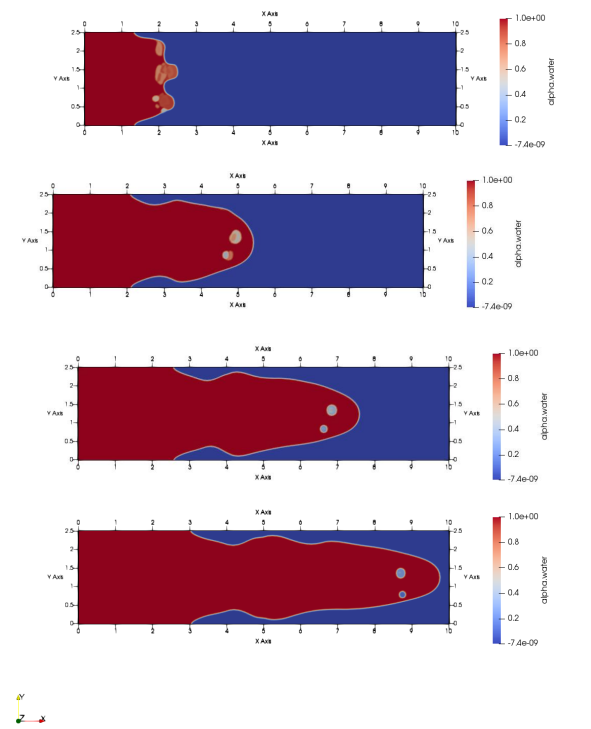
\includegraphics[width=0.85\linewidth]{saffman-001.png}
\captionof{figure}{A simulation of the Saffman–Taylor instability is performed in \textbf{OpenFOAM} within a 10\,m $\times$ 2.5\,m $\times$ 0.01\,m Hele-Shaw cell initially filled with oil \textcolor{blue}{(blue)}. Water \textcolor{red}{(red)} is injected at the inlet, triggering viscous fingering due to a high mobility ratio, $\mu_{\text{oil}} / \mu_{\text{water}} = 3000$. Snapshots at 80\,s, 320\,s, 480\,s, and 640\,s show the progression and growth of the instability. Gravity effects are neglected and a surface tension coefficient of 0.006\,N/m is used.}

\label{fig:saffman-instability}
\end{figure}

\begin{figure}[H]
\centering
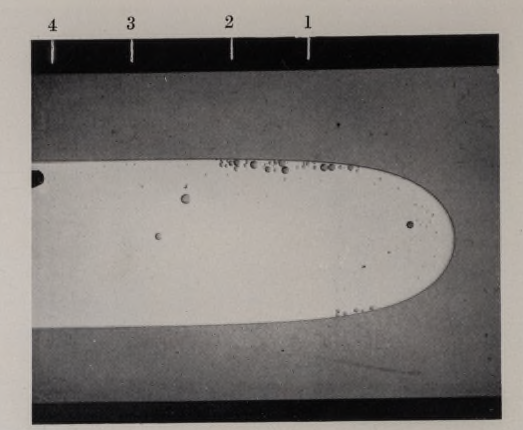
\includegraphics[width=\linewidth]{Finger_001.png}
\captionof{figure}{Finger of oil (\( \mu = 4.5\,\text{P} \)) penetrating glycerine (\( \mu = 9\,\text{P} \)) in a Hele-Shaw cell. Image adapted from~\cite{SaffmanTaylor1958}.}

\label{fig:saffman-instability-finger}

\end{figure}
\end{multicols} 

\newpage

\begin{multicols}{2}
The growth of these fingers is not liner but rather in complex fractal patterns to maximize the interfacial surface area.The \textit{Young-Laplace} equation has an important role in establishing the relationship between pressure difference across fluid interfaces and their geometric properties. Its defined as \[
\Delta p = \gamma \left( \frac{1}{R_1} + \frac{1}{R_2} \right)
\]
this boundary condition is useful for solving the \textit{\textbf{Laplace equation}} for pressure within the domain.


\end{multicols}
\subsection{Radial and Linear viscous Fingering}
\begin{figure}[H]
  \centering

  % Row 1
  \begin{subfigure}{0.45\linewidth}
    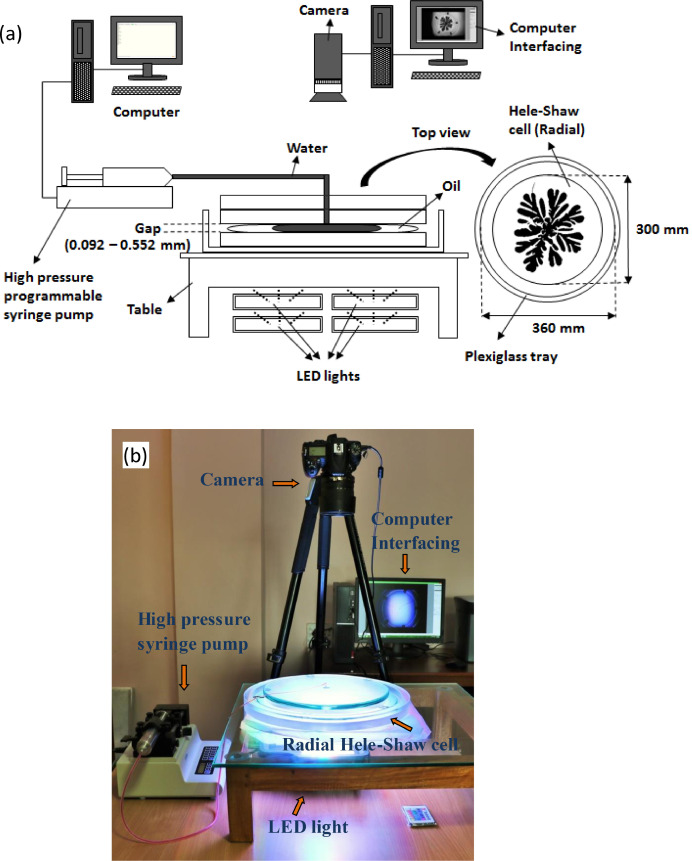
\includegraphics[width=0.8\linewidth]{aparatus-002.jpg}
    \caption{Experimental setup: (a) schematic and photograph of the radial Hele–Shaw cell with syringe pump, LED illumination, and camera interface.}
  \end{subfigure}
  \hfill
  \begin{subfigure}{0.45\linewidth}
    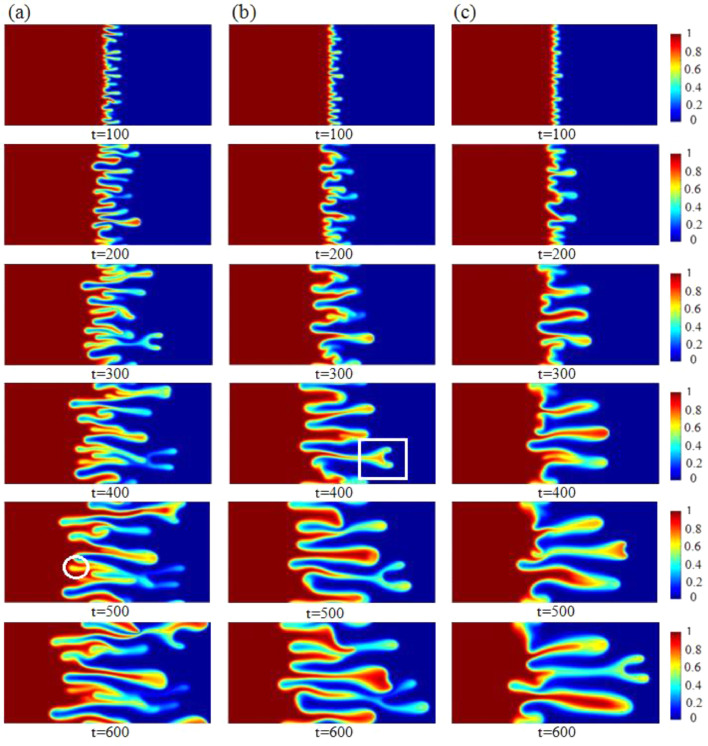
\includegraphics[width=0.9\linewidth]{1-s2.0-S0020740317306422-linaer.jpg}
    \caption{Linear viscous fingering in a rectilinear channel showing tip–splitting and side branching at fixed flow rate.}
  \end{subfigure}

  % Row 2
  \begin{subfigure}{0.45\linewidth}
    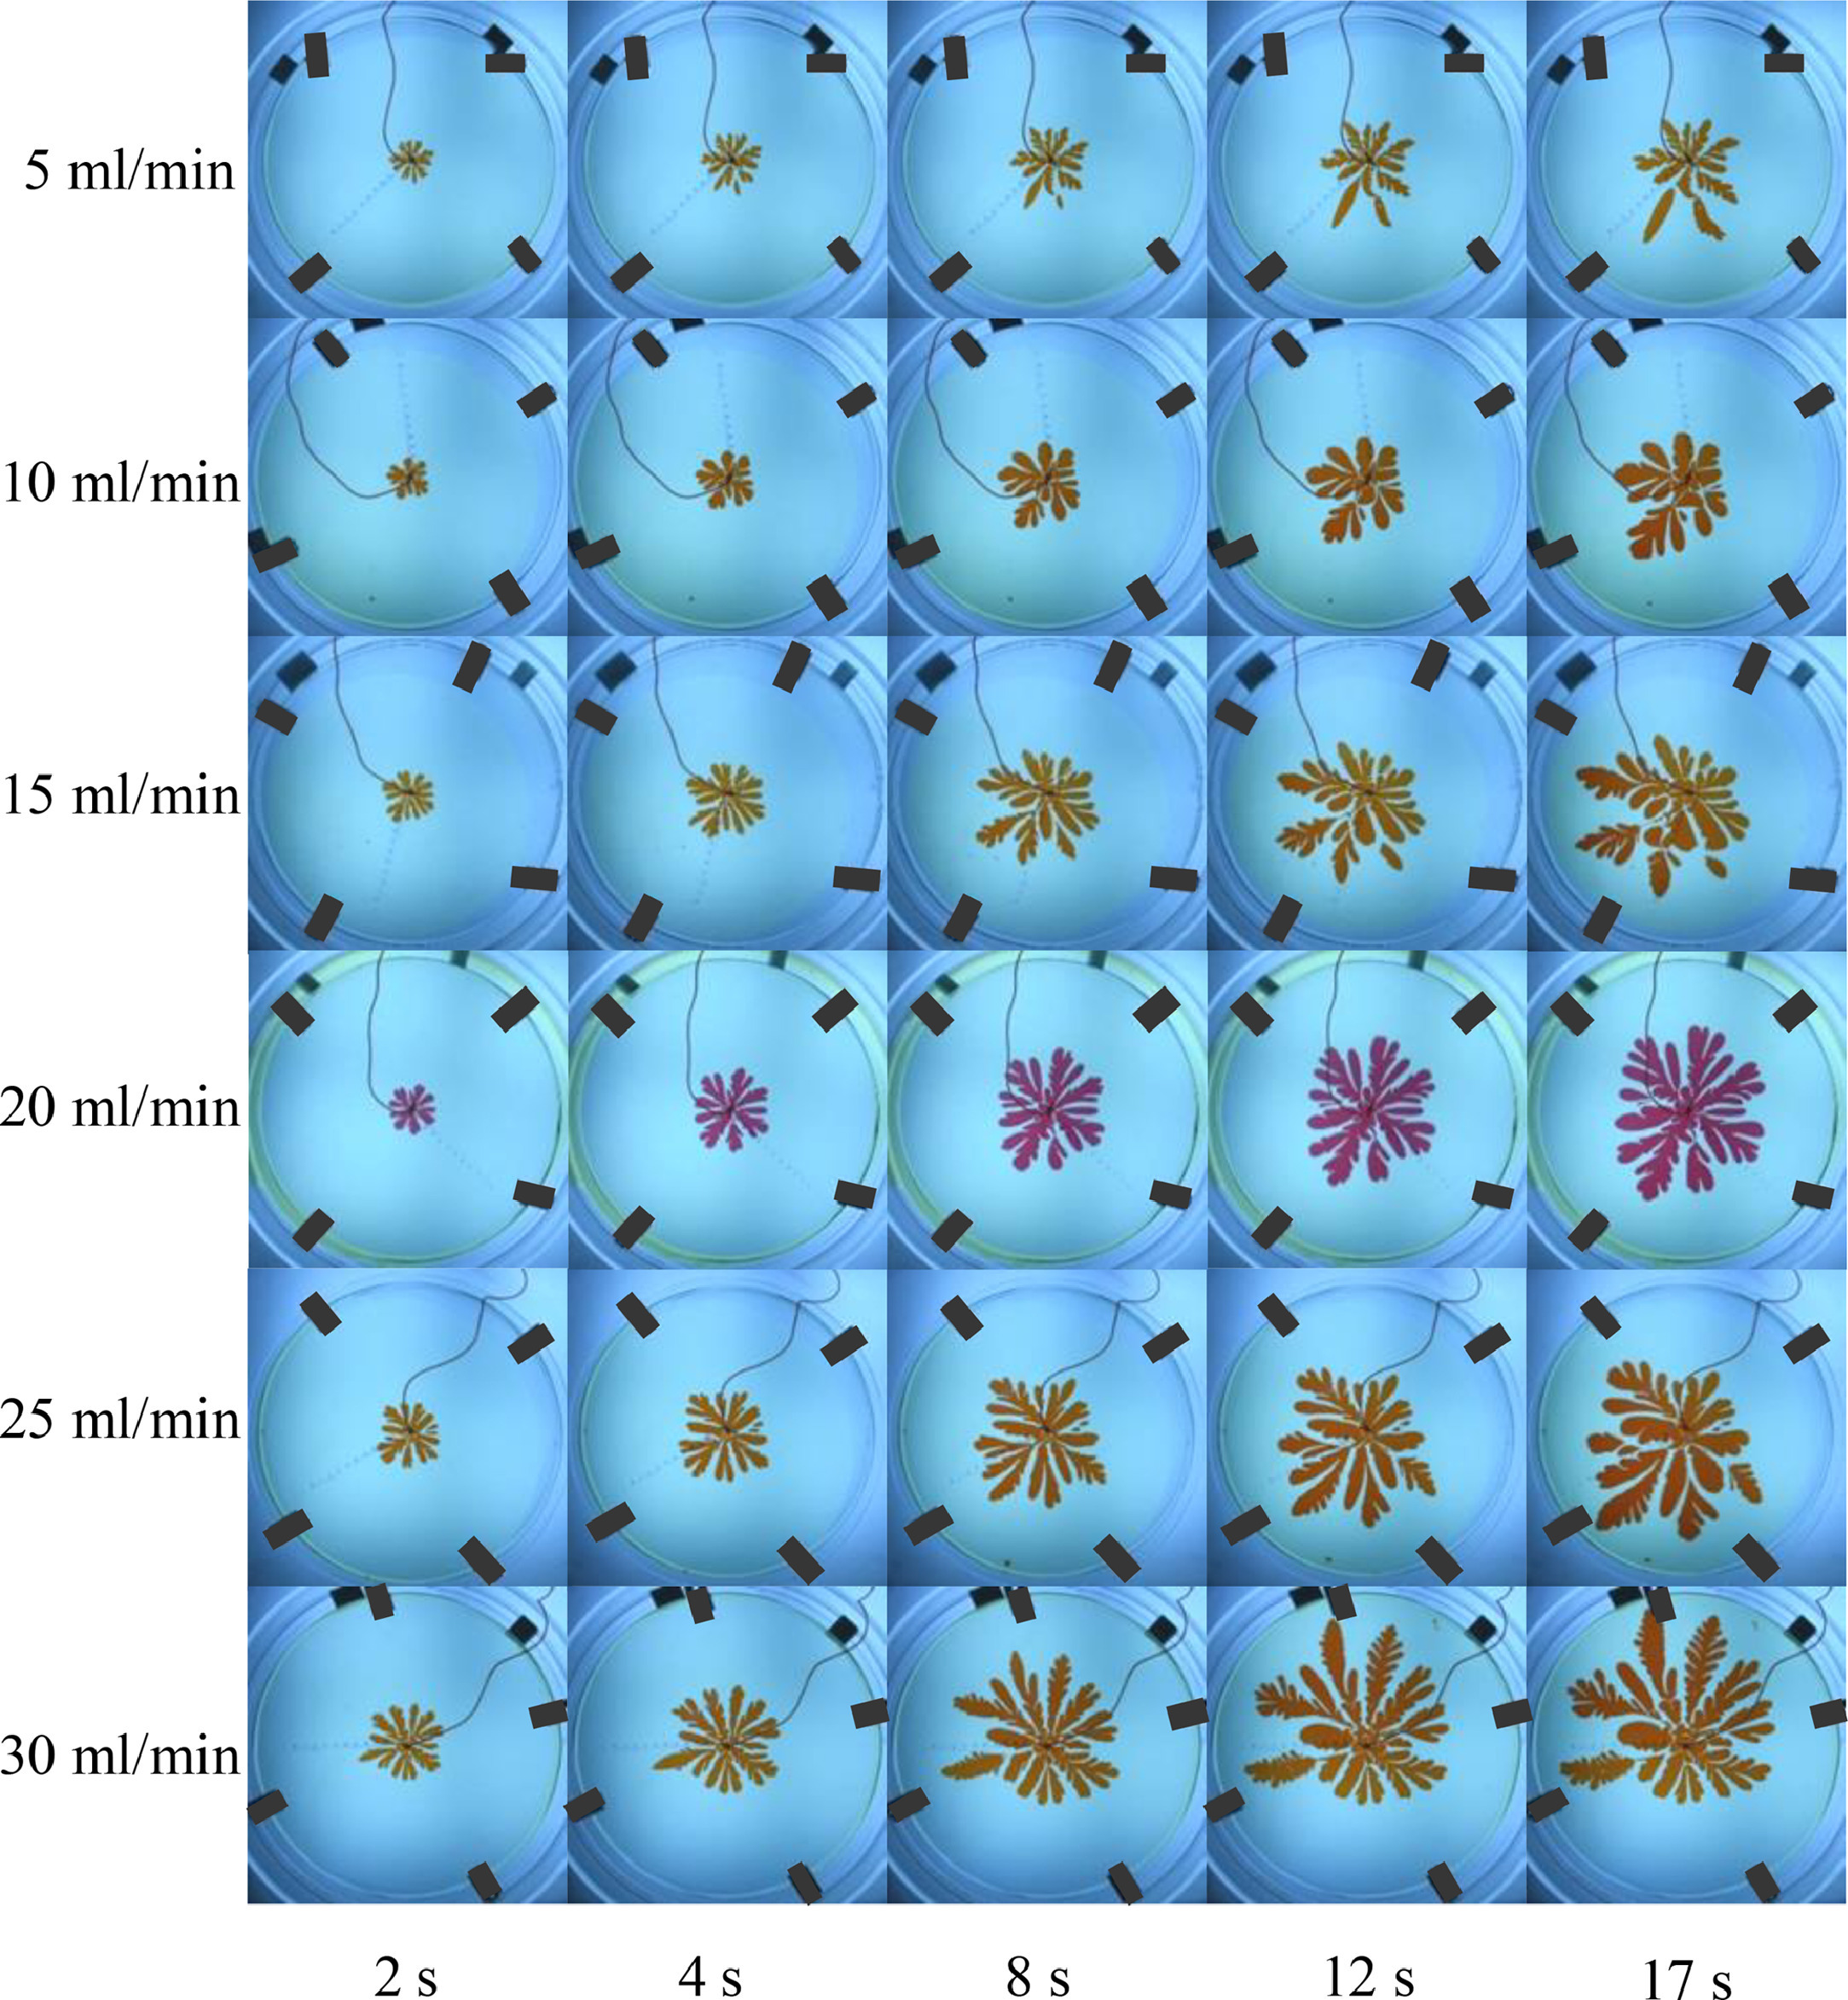
\includegraphics[width=0.9\linewidth]{raates-sft-004.jpg}
\caption{Radial fingering snapshots at various times (2–17 s) and flow rates (5–30 mL \( \mathrm{min}^{-1} \)), illustrating rate‐dependent branching.}

  \end{subfigure}
  \hfill
  \begin{subfigure}{0.45\linewidth}
    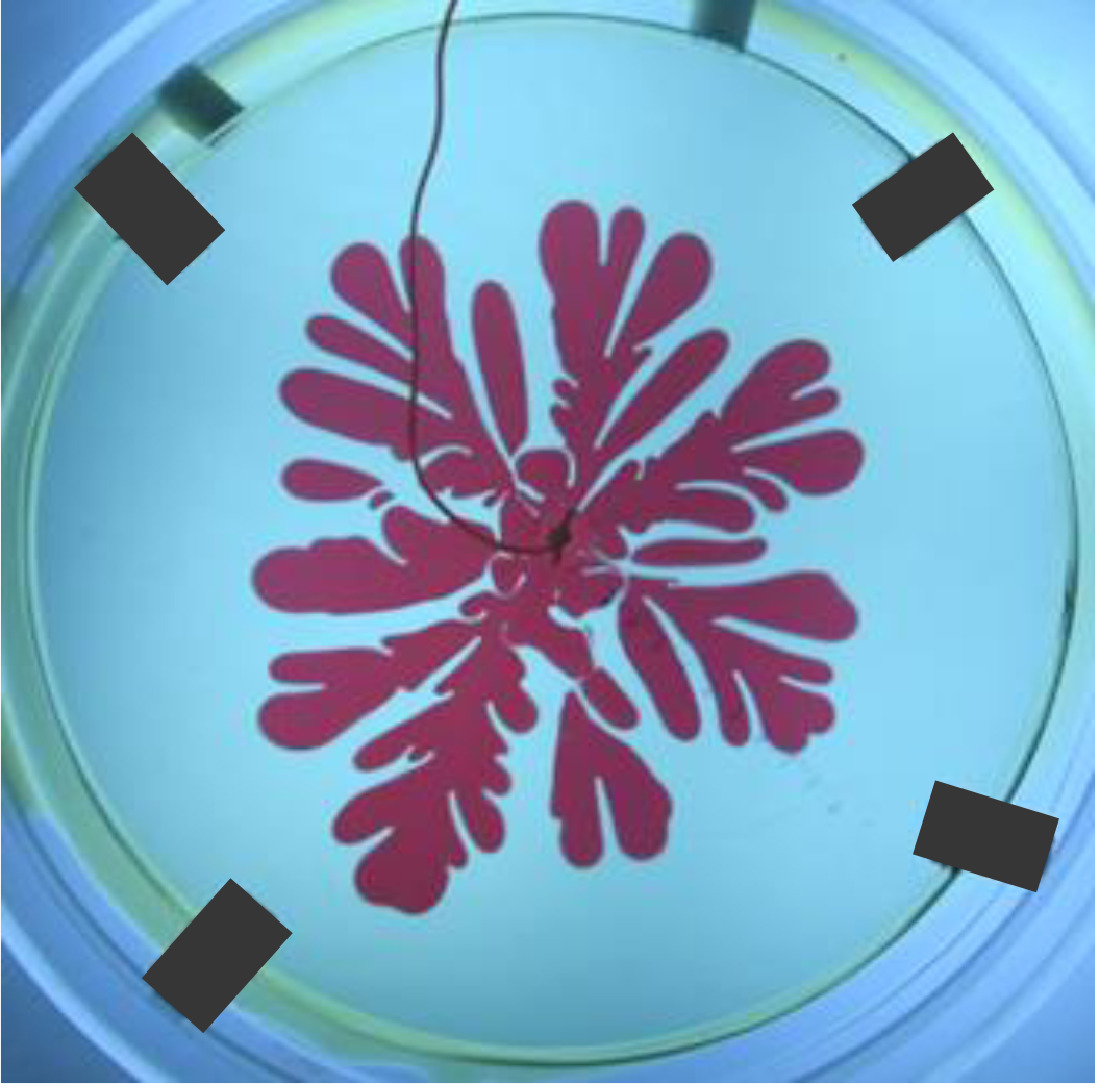
\includegraphics[width=0.8\linewidth]{high-res-sft-003.jpg}
    \caption{Late‐time viscous finger morphology of dyed water (pink) in oil at ultra-low injection rate, showing detachment and secondary branching.}
  \end{subfigure}

  \caption[Viscous fingering in a radial Hele–Shaw cell]{%
    Viscous fingering patterns in a radial Hele–Shaw cell (gap = 0.092 mm), invading fluid: dyed water, displaced fluid: gear oil (SAE 85W-140), adapted from \cite{singh2021saffman} \cite{shokri2018saffman}.%
  }
  \label{fig:grid}
\end{figure}


\newpage
\section{Hele-Shaw Cells}
\begin{minipage}[t]{0.5\textwidth}
\vspace{0pt} 

The Hele-Shaw cell is named after \textit{Henry Selby Hele-Shaw}, a British mechanical engineer who first introduced this apparatus in 1898. \\

These cells provide us an apparatus to perform clean ,controlled setting of viscous dominated and quasi two-dimensional fluid dynamics experiments.The Hele-Shaw cell consists of two closely spaced plates with the gap between them ($h \ll L$) which is small enough so that motion of the fluid is essentially confined to the horizontal plane. \\



\end{minipage}
\hfill
\begin{minipage}[t]{0.45\textwidth}
\centering
\vspace{0pt} 
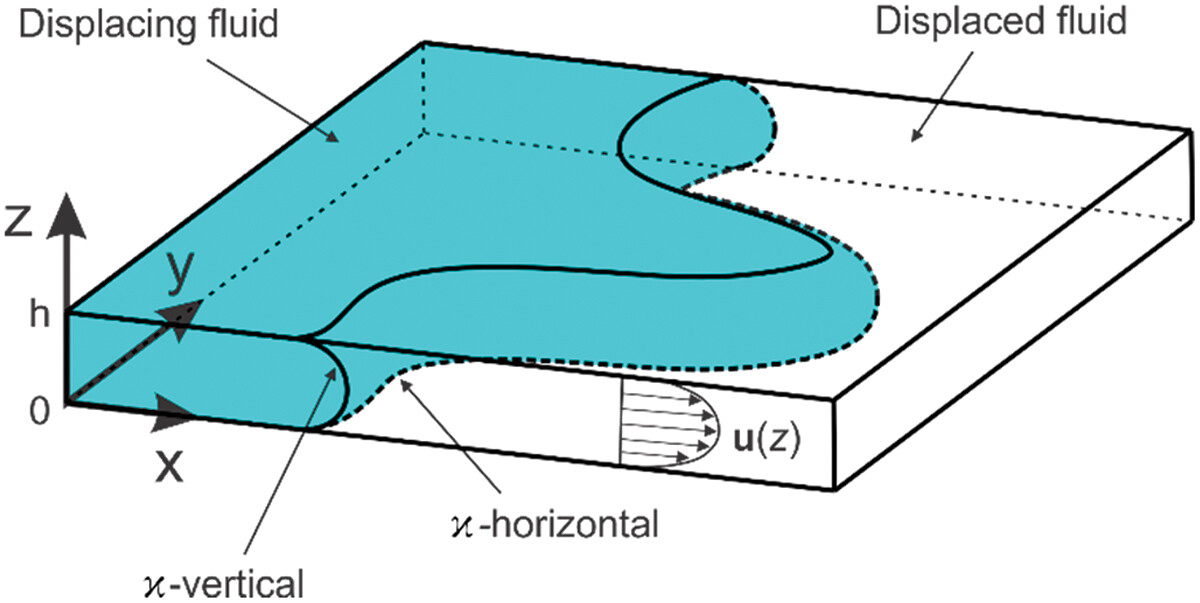
\includegraphics[width=0.95\linewidth]{hele-shaw-002.jpg}
\captionof{figure}{The Hele-Shaw flow in a planar channel geometry within the frame of reference.\\
Adapted from \textit{Journal of the Indian Institute of Science}, Saffman–Taylor Instability: Linear Stability Analysis and Beyond, \cite{mahato2024saffman}.}
\label{fig:hele-shaw}
\end{minipage}
The velocity of fluid flow inside the Hele-Shaw cell is typically slow and therefore ensure a low Reynolds number regime ($Re \ll 1$), where viscous forces are dominant over inertial effects.As a result, the flow remains laminar.The no-slip condition at both plates creates a parabolic velocity profile across the gap, which can be averaged to yield $u_{avg}$.

\subsection{Mathematical Explanation for Linear Hele-Shaw flow}

We know the Navier-Stokes equations for an incompressible flow:
\begin{mdframed}[linewidth=0.5pt]
\begin{equation}
\rho \left( \frac{\partial \mathbf{v}}{\partial t} + (\mathbf{v} \cdot \nabla) \mathbf{v} \right) = -\nabla p + \mu \nabla^2 \mathbf{v} + \mathbf{F}
\end{equation}
\end{mdframed}
and the continuity equation:
\begin{equation}
\nabla \cdot \mathbf{v} = 0
\end{equation}

where $\rho$ is fluid density, $\mathbf{v}$ is velocity vector, $p$ is pressure, $\mu$ is dynamic viscosity, and $\mathbf{F}$ represents body forces (e.g., gravity).
In Cartesian coordinates, these equations expand to:


\begin{align}
\rho \left( \frac{\partial u}{\partial t} + u\frac{\partial u}{\partial x} + v\frac{\partial u}{\partial y} + w\frac{\partial u}{\partial z} \right) &= -\frac{\partial p}{\partial x} + \mu \left( \frac{\partial^2 u}{\partial x^2} + \frac{\partial^2 u}{\partial y^2} + \frac{\partial^2 u}{\partial z^2} \right) + F_x \\
\rho \left( \frac{\partial v}{\partial t} + u\frac{\partial v}{\partial x} + v\frac{\partial v}{\partial y} + w\frac{\partial v}{\partial z} \right) &= -\frac{\partial p}{\partial y} + \mu \left( \frac{\partial^2 v}{\partial x^2} + \frac{\partial^2 v}{\partial y^2} + \frac{\partial^2 v}{\partial z^2} \right) + F_y \\
\rho \left( \frac{\partial w}{\partial t} + u\frac{\partial w}{\partial x} + v\frac{\partial w}{\partial y} + w\frac{\partial w}{\partial z} \right) &= -\frac{\partial p}{\partial z} + \mu \left( \frac{\partial^2 w}{\partial x^2} + \frac{\partial^2 w}{\partial y^2} + \frac{\partial^2 w}{\partial z^2} \right) + F_z
\end{align}



and the continuity equation:
\begin{equation}
\frac{\partial u}{\partial x} + \frac{\partial v}{\partial y} + \frac{\partial w}{\partial z} = 0
\end{equation}
where $(u, v, w)$ are the velocity components in the $(x, y, z)$ directions.

\subsection{Boundary Conditions in Hele-Shaw Flows}
\begin{enumerate}
  \item \textbf{Gap width:} The gap width \(h\) is much smaller than the characteristic length scale \(L\) in \(x\)-\(y\) plane,which indicates \(h \ll L\). Because of this the fluid is confined to a very thin gap and therefore the velocity gradients in the \(z\)-direction dominate over the variations in \(x\) or \(y\) directions.

  \item \textbf{Low Reynolds number:} The velocity of flow is very slow, which means the flow has low Reynolds number: 
    \[
      Re = \frac{\rho U L}{\mu} \ll 1,
    \]
    where \(U\) is a characteristic velocity. With viscous forces dominating, the  \\ 
    \(\rho\,\mathbf{v}\cdot\nabla\mathbf{v}\) term in the Navier–Stokes equation becomes negligible and hence we drop it.

  \item \textbf{No-slip at plates:} No-slip boundary conditions applied at both ends of the plates: \(\mathbf{v} = 0\) at \(z = 0\) and \(z = h\).

  \item \textbf{Predominantly 2D flow:} The flow is  two-dimensional in the \(x\)-\(y\) plane so vertical velocity \(w\) is negligible.Therefore we can drop the \(w\)-component of velocity.

  \item \textbf{Horizontal pressure variation:} The pressure \(p\) varies primarily in the \(x\)-\(y\) plane and not in the \(z\)-direction.So we can drop the \(\partial p / \partial z\) terms in the vertical momentum equation.
\end{enumerate}

after applying the above boundary conditions the equation reduces to : 

\[
\boxed{
    \nabla p = \mu \nabla^2 \mathbf{v} + \mathbf{F}
}
\]




Derivation of the Laplace Equation for Pressure,
\begin{align}
    -\frac{h^2}{12\mu}\nabla_{xy} \cdot (\nabla_{xy} p) + \frac{h^2}{12\mu}\nabla_{xy} \cdot \mathbf{F}_{xy} = 0
\end{align}

Recognizing that $\nabla_{xy} \cdot (\nabla_{xy} p) = \nabla^2_{xy} p$, which is the Laplacian of pressure:
\begin{align}
    -\frac{h^2}{12\mu}\nabla^2_{xy} p + \frac{h^2}{12\mu}\nabla_{xy} \cdot \mathbf{F}_{xy} = 0
\end{align}

In the absence of body forces ($\mathbf{F}_{xy} = \mathbf{0}$) the equation simplifies to:
\begin{align}
    -\frac{h^2}{12\mu}\nabla^2_{xy} p = 0
\end{align}

Since $\frac{h^2}{12\mu}$ is a non-zero constant coefficient, we have:
\[
\boxed{
    \nabla^2_{xy} p = 0
}
\]

In a Hele-Shaw cell, the pressure follows something called the Laplace equation when there are no sources or sinks (like places where fluid is added or removed). This just means the pressure behaves in a smooth and balanced way. It doesn’t have any sharp peaks or dips inside the flow area and no local highs or lows. At any point, the pressure is basically an average of the pressure around it. Also, if we know the pressure along the edges or boundaries of the region, we can figure out the pressure everywhere else inside.

\subsection{Linear velocity in Hele-Shaw cell for  viscous Fingering}

\subsubsection*{Applying Hele-Shaw Assumptions}

For a Hele-Shaw cell with gap width $b \ll L$, velocity gradients in the $z$-direction dominate:
\begin{equation}
 \begin{aligned}
    \frac{\partial^2 u}{\partial z^2} \gg \frac{\partial^2 u}{\partial x^2}, \frac{\partial^2 u}{\partial y^2} 
    \hspace{2cm}
    \frac{\partial^2 v}{\partial z^2} \gg \frac{\partial^2 v}{\partial x^2}, \frac{\partial^2 v}{\partial y^2}
\end{aligned}   
\end{equation}


Since pressure varies primarily in the $x$-$y$ plane, $\frac{\partial p}{\partial z} \approx 0$. 
This simplifies our momentum equations to:
\begin{equation}
\begin{aligned}
    \frac{\partial p}{\partial x} &= \mu \frac{\partial^2 u}{\partial z^2} + F_x \hspace{2cm}
    \frac{\partial p}{\partial y} &= \mu \frac{\partial^2 v}{\partial z^2} + F_y
\end{aligned}
\end{equation}

    

\subsubsection*{Solving for Velocity Profiles}

Rearranging to isolate the second derivatives:
\begin{align}
    \frac{\partial^2 u}{\partial z^2} &= \frac{1}{\mu}\left(\frac{\partial p}{\partial x} - F_x\right) \\
    \frac{\partial^2 v}{\partial z^2} &= \frac{1}{\mu}\left(\frac{\partial p}{\partial y} - F_y\right)
\end{align}

Integrating twice with respect to $z$ for $u$:
\begin{align}
    \frac{\partial u}{\partial z} &= \frac{1}{\mu}\left(\frac{\partial p}{\partial x} - F_x\right)z + C_1 \\
    u(z) &= \frac{1}{2\mu}\left(\frac{\partial p}{\partial x} - F_x\right)z^2 + C_1 z + C_2
\end{align}

Applying no-slip boundary conditions at $z=0$ and $z=h$:
\begin{align}
    u(0) &= 0 \implies C_2 = 0 \\
    u(h) &= 0 \implies \frac{1}{2\mu}\left(\frac{\partial p}{\partial x} - F_x\right)h^2 + C_1 h = 0 \\
    \implies C_1 &= -\frac{h}{2\mu}\left(\frac{\partial p}{\partial x} - F_x\right)
\end{align}

Substituting these constants:
\begin{align}
    u(z) &= \frac{1}{2\mu}\left(\frac{\partial p}{\partial x} - F_x\right)z^2 - \frac{h}{2\mu}\left(\frac{\partial p}{\partial x} - F_x\right)z \\
    &= \frac{1}{2\mu}\left(\frac{\partial p}{\partial x} - F_x\right)z(z-h) \\
    &= \frac{1}{2\mu}\left(F_x - \frac{\partial p}{\partial x}\right)z(h-z)
\end{align}

Similarly for $v(z)$:
\begin{align}
    v(z) = \frac{1}{2\mu}\left(F_y - \frac{\partial p}{\partial y}\right)z(h-z)
\end{align}

\subsubsection*{Depth-Averaged Velocities}

To obtain depth-averaged velocities, we integrate over the gap height:
\begin{align}
    \bar{u} &= \frac{1}{h}\int_0^h u(z) dz \\
    &= \frac{1}{h}\int_0^h \frac{1}{2\mu}\left(F_x - \frac{\partial p}{\partial x}\right)z(h-z) dz \\
    &= \frac{1}{2\mu h}\left(F_x - \frac{\partial p}{\partial x}\right)\int_0^h (hz - z^2) dz \\
    &= \frac{1}{2\mu h}\left(F_x - \frac{\partial p}{\partial x}\right)\left[\frac{hz^2}{2} - \frac{z^3}{3}\right]_0^h \\
    &= \frac{1}{2\mu h}\left(F_x - \frac{\partial p}{\partial x}\right)\left(\frac{h^3}{2} - \frac{h^3}{3}\right) \\
    &= \frac{1}{2\mu h}\left(F_x - \frac{\partial p}{\partial x}\right)\frac{h^3}{6} \\
    &= \frac{h^2}{12\mu}\left(F_x - \frac{\partial p}{\partial x}\right)
\end{align}

Similarly for $\bar{v}$:
\begin{align}
    \bar{v} = \frac{h^2}{12\mu}\left(F_y - \frac{\partial p}{\partial y}\right)
\end{align}

\subsubsection*{Final Depth-Averaged Velocity Equations}

Rearranging to standard form:
\begin{equation}
   \begin{aligned}
    \bar{u} &= -\frac{h^2}{12\mu}\frac{\partial p}{\partial x} + \frac{h^2}{12\mu}F_x 
    \hspace{2cm}
    \bar{v} &= -\frac{h^2}{12\mu}\frac{\partial p}{\partial y} + \frac{h^2}{12\mu}F_y
\end{aligned}
\end{equation}

Or in vector notation:
\begin{align}
    \bar{\mathbf{u}} = -\frac{h^2}{12\mu}\nabla_{xy} p + \frac{h^2}{12\mu}\mathbf{F}_{xy}
\end{align}

Where $\bar{\mathbf{u}} = (\bar{u}, \bar{v})$ is the depth-averaged velocity vector, $\nabla_{xy}$ is the gradient operator in the $x$-$y$ plane, and $\mathbf{F}_{xy} = (F_x, F_y)$ is the horizontal body force.

If we consider body forces $\mathbf{F}_{xy}$ to be negligible,then the averaged velocities:
\begin{mdframed}[linewidth=0.5pt]
\begin{align}
    \bar{\mathbf{u}} = -\frac{h^2}{12\mu}\nabla_{xy} p 
\end{align}
\end{mdframed}

% only viscous 

% \begin{mdframed}[linewidth=0.5pt]
% % Add experimental setup details here
% \end{mdframed}



This form is equivalent to\textbf{ Darcy's law} \cite{Whitaker1986}, which says that the flow through porous media:
\begin{align}
    \mathbf{q} = -\frac{k}{\mu}\nabla p
\end{align}
where $\mathbf{q}$ is the Darcy flux (volume flow rate per unit area),and  $k$ is the permeability and $\mu$ is the viscosity of the fluid .Comparing these equations reveals that a Hele-Shaw cell effectively models a porous medium with permeability:
\begin{mdframed}
  \begin{align}
    k = \frac{h^2}{12}
\end{align}  
\end{mdframed}

\subsection{Limitations}
The Hele-Shaw cell is one of the useful tool for modeling flow through a porous media, but it does come with few limitations.It assumes the permeability is the same in all directions (isotropic permeability) which isn’t always true in general. Actual porous media have complex, irregular pore structures that can’t be accurately captured by the simple setup of two flat closely placed plates. It also falls back when trying to demonstrate more complicated behaviors, like how different fluids interact and move through a real porous network. Finally, the Hele-Shaw approach only works well for very slow, viscous flows, so it doesn't apply when the flow gets faster or turbulent (Laminar Regime).


\section{Applications}
\subsection{Enhanced Oil Recovery}
% Add oil recovery applications here HUMANIZE 
During the crude oil extraction process,water is injected to displace the more viscous oil that is collected at the tanks situated at the ground.during this the less viscous water water pushes the oil interface and the Saffman-Taylor instability creates finger like water channels in the oil.these fingers grow and cause premature water breakthrough at the collection wells often leaving behind 50\% oil.This increases the barrel cost due to expensive  separation process.To avoid this we often add polymer derivatives to keep mobility ratios around 5:1.As reservoirs  are becoming increasingly complex and hydrocarbons extraction is shifting towards heavier oils, mastering the Saffman-Taylor instability will remain important for balancing the operational efficiency along with environmental and economic sustainability.



\section{Numerical Modeling and Conclusion}

We also analyse the Hele-shaw flow in radial geometry, which also has similar approach.There are also inclusions of effect of gravity.For real life analytical solutions we consider the wavelength of fingers and also the oscillations of the perturbation near the injecting fluid area which decides whether the fingers split or not.All of these topics are out of this reports view and are mentioned in the below attached references

The \textbf{openFOAM simulation for Linear Hele Shaw flow} is done and the code files are attached in the \textbf{GitHub} repository .Also the Tex files for this report are available. I have also made the video for the simulation.
% Add numerical modeling information here

\begin{mdframed}[linewidth=0.5pt]
% Add conclusion and future directions here
\begin{align}
  {\href{https://github.com/Akshit11318/MM2041_REPORT.git}{\textit{\textbf{https://github.com/Akshit11318/MM2041\_REPORT.git}}}}  
\end{align}
\end{mdframed}


\newpage
\begin{thebibliography}{09}
% Add your references here
\bibitem{SaffmanTaylor1958}
P.~G. Saffman and G.~I. Taylor,
``The penetration of a fluid into a porous medium or Hele-Shaw cell containing a more viscous liquid,''
\emph{Proceedings of the Royal Society of London. Series A. Mathematical and Physical Sciences}, vol.~245, no.~1242, pp.~312--329, 1958. doi: \href{https://doi.org/10.1098/rspa.1958.0085}{10.1098/rspa.1958.0085}.

\bibitem{HeleShaw1898}
HELE-SHAW, H. S. (1898). The Flow of Water. Nature, 58(1489), 34–36. \href{https://doi.org/10.1038/058034a0}{10.1038/058034a0}

\bibitem{Saffman1986}
P.~G. Saffman, ``Viscous fingering in Hele-Shaw cells,'' \emph{Journal of Fluid Mechanics}, vol.~173, pp.~73--94, 1986. doi: \href{https://doi.org/10.1017/S0022112086001088}{10.1017/S0022112086001088}.

\bibitem{Lenormand1988}
Lenormand, R., Touboul, E., \& Zarcone, C. (1988). Numerical models and experiments on immiscible displacements in porous media. \textit{Journal of Fluid Mechanics}, \textit{189}, 165--187. \href{https://doi.org/10.1017/S0022112088000953}{doi:10.1017/S0022112088000953}



\bibitem{mahato2024saffman}
Diptesh Mahato and Manoranjan Mishra,
\textit{Saffman--Taylor Instability: Linear Stability Analysis and Beyond},
Journal of the Indian Institute of Science, 2024. 
DOI: \href{https://doi.org/10.1080/23746149.2024.2370838}{10.1080/23746149.2024.2370838}.

\bibitem{Whitaker1986}
S. Whitaker,
\emph{Flow in porous media I: A theoretical derivation of Darcy’s law},
Transport in Porous Media, vol. 1, no. 1, pp. 3–25, Mar. 1986.
doi: \href{https://doi.org/10.1007/BF01036523}{10.1007/BF01036523}.

\bibitem{sheng2010modern}
Sheng, J. J. (2010). \textit{Modern chemical enhanced oil recovery: theory and practice}. Gulf Professional Publishing.

\bibitem{Bublik2021}
Bublik, S.A. and Semin, M.A. (2021). Study of the Saffman–Taylor Instability in an Oil Reservoir Formation in Two Dimensions. \textit{Mathematical Models and Computer Simulations}, 13, 263–273. https://doi.org/10.1134/S2070048221020046


\bibitem{PhysRevA.31.1977}
Tang, C. (1985). Diffusion-limited aggregation and the Saffman-Taylor problem. \textit{Physical Review A}, \textit{31}(3), 1977--1979. \href{https://doi.org/10.1103/PhysRevA.31.1977}{doi:10.1103/PhysRevA.31.1977}

\bibitem{article}
Lagrée, B., Zaleski, S., Bondino, I., Josserand, C., \& Popinet, S. (2014, October). Scaling properties of viscous fingering. \textit{arXiv:1410.8659 [physics.flu-dyn]}. \url{https://arxiv.org/abs/1410.8659}

\bibitem{singh2021saffman}
Singh, P., Ramisetti, L., \& Mondal, S. (2021). Saffman-Taylor instability in a radial Hele-Shaw cell for a shear-dependent rheological fluid. \textit{Journal of Non-Newtonian Fluid Mechanics}, \textit{294}, 104579. \href{https://doi.org/10.1016/j.jnnfm.2021.104579}{doi:10.1016/j.jnnfm.2021.104579}


\bibitem{shokri2018saffman}
H. Shokri, M.~H. Kayhani, and M. Norouzi,
``Saffman–Taylor instability of viscoelastic fluids in anisotropic porous media,''
\textit{International Journal of Mechanical Sciences}, vol. 135, pp. 1--13, 2018.
\href{https://doi.org/10.1016/j.ijmecsci.2017.11.008}{doi:10.1016/j.ijmecsci.2017.11.008}.


\bibitem{singh2021cfd}
A. Singh, K.~M. Pandey, and Y. Singh,
``CFD analysis of viscous fingering in Hele-Shaw cell for air-glycerin system,''
\textit{Materials Today: Proceedings}, vol. 45, part 7, pp. 6381--6385, 2021.
\href{https://doi.org/10.1016/j.matpr.2020.11.069}{doi:10.1016/j.matpr.2020.11.069}.


\bibitem{paterson1981radial}
Paterson, L. (1981). Radial fingering in a Hele Shaw cell. \textit{Journal of Fluid Mechanics}, \textit{113}, 513--529. \href{https://doi.org/10.1017/S0022112081003613}{doi:10.1017/S0022112081003613}



\end{thebibliography}

\end{document}